
% Default to the notebook output style

    


% Inherit from the specified cell style.




    
\documentclass[11pt]{article}

    
    
    \usepackage[T1]{fontenc}
    % Nicer default font (+ math font) than Computer Modern for most use cases
    \usepackage{mathpazo}

    % Basic figure setup, for now with no caption control since it's done
    % automatically by Pandoc (which extracts ![](path) syntax from Markdown).
    \usepackage{graphicx}
    % We will generate all images so they have a width \maxwidth. This means
    % that they will get their normal width if they fit onto the page, but
    % are scaled down if they would overflow the margins.
    \makeatletter
    \def\maxwidth{\ifdim\Gin@nat@width>\linewidth\linewidth
    \else\Gin@nat@width\fi}
    \makeatother
    \let\Oldincludegraphics\includegraphics
    % Set max figure width to be 80% of text width, for now hardcoded.
    \renewcommand{\includegraphics}[1]{\Oldincludegraphics[width=.8\maxwidth]{#1}}
    % Ensure that by default, figures have no caption (until we provide a
    % proper Figure object with a Caption API and a way to capture that
    % in the conversion process - todo).
    \usepackage{caption}
    \DeclareCaptionLabelFormat{nolabel}{}
    \captionsetup{labelformat=nolabel}

    \usepackage{adjustbox} % Used to constrain images to a maximum size 
    \usepackage{xcolor} % Allow colors to be defined
    \usepackage{enumerate} % Needed for markdown enumerations to work
    \usepackage{geometry} % Used to adjust the document margins
    \usepackage{amsmath} % Equations
    \usepackage{amssymb} % Equations
    \usepackage{textcomp} % defines textquotesingle
    % Hack from http://tex.stackexchange.com/a/47451/13684:
    \AtBeginDocument{%
        \def\PYZsq{\textquotesingle}% Upright quotes in Pygmentized code
    }
    \usepackage{upquote} % Upright quotes for verbatim code
    \usepackage{eurosym} % defines \euro
    \usepackage[mathletters]{ucs} % Extended unicode (utf-8) support
    \usepackage[utf8x]{inputenc} % Allow utf-8 characters in the tex document
    \usepackage{fancyvrb} % verbatim replacement that allows latex
    \usepackage{grffile} % extends the file name processing of package graphics 
                         % to support a larger range 
    % The hyperref package gives us a pdf with properly built
    % internal navigation ('pdf bookmarks' for the table of contents,
    % internal cross-reference links, web links for URLs, etc.)
    \usepackage{hyperref}
    \usepackage{longtable} % longtable support required by pandoc >1.10
    \usepackage{booktabs}  % table support for pandoc > 1.12.2
    \usepackage[inline]{enumitem} % IRkernel/repr support (it uses the enumerate* environment)
    \usepackage[normalem]{ulem} % ulem is needed to support strikethroughs (\sout)
                                % normalem makes italics be italics, not underlines
    

    
    
    % Colors for the hyperref package
    \definecolor{urlcolor}{rgb}{0,.145,.698}
    \definecolor{linkcolor}{rgb}{.71,0.21,0.01}
    \definecolor{citecolor}{rgb}{.12,.54,.11}

    % ANSI colors
    \definecolor{ansi-black}{HTML}{3E424D}
    \definecolor{ansi-black-intense}{HTML}{282C36}
    \definecolor{ansi-red}{HTML}{E75C58}
    \definecolor{ansi-red-intense}{HTML}{B22B31}
    \definecolor{ansi-green}{HTML}{00A250}
    \definecolor{ansi-green-intense}{HTML}{007427}
    \definecolor{ansi-yellow}{HTML}{DDB62B}
    \definecolor{ansi-yellow-intense}{HTML}{B27D12}
    \definecolor{ansi-blue}{HTML}{208FFB}
    \definecolor{ansi-blue-intense}{HTML}{0065CA}
    \definecolor{ansi-magenta}{HTML}{D160C4}
    \definecolor{ansi-magenta-intense}{HTML}{A03196}
    \definecolor{ansi-cyan}{HTML}{60C6C8}
    \definecolor{ansi-cyan-intense}{HTML}{258F8F}
    \definecolor{ansi-white}{HTML}{C5C1B4}
    \definecolor{ansi-white-intense}{HTML}{A1A6B2}

    % commands and environments needed by pandoc snippets
    % extracted from the output of `pandoc -s`
    \providecommand{\tightlist}{%
      \setlength{\itemsep}{0pt}\setlength{\parskip}{0pt}}
    \DefineVerbatimEnvironment{Highlighting}{Verbatim}{commandchars=\\\{\}}
    % Add ',fontsize=\small' for more characters per line
    \newenvironment{Shaded}{}{}
    \newcommand{\KeywordTok}[1]{\textcolor[rgb]{0.00,0.44,0.13}{\textbf{{#1}}}}
    \newcommand{\DataTypeTok}[1]{\textcolor[rgb]{0.56,0.13,0.00}{{#1}}}
    \newcommand{\DecValTok}[1]{\textcolor[rgb]{0.25,0.63,0.44}{{#1}}}
    \newcommand{\BaseNTok}[1]{\textcolor[rgb]{0.25,0.63,0.44}{{#1}}}
    \newcommand{\FloatTok}[1]{\textcolor[rgb]{0.25,0.63,0.44}{{#1}}}
    \newcommand{\CharTok}[1]{\textcolor[rgb]{0.25,0.44,0.63}{{#1}}}
    \newcommand{\StringTok}[1]{\textcolor[rgb]{0.25,0.44,0.63}{{#1}}}
    \newcommand{\CommentTok}[1]{\textcolor[rgb]{0.38,0.63,0.69}{\textit{{#1}}}}
    \newcommand{\OtherTok}[1]{\textcolor[rgb]{0.00,0.44,0.13}{{#1}}}
    \newcommand{\AlertTok}[1]{\textcolor[rgb]{1.00,0.00,0.00}{\textbf{{#1}}}}
    \newcommand{\FunctionTok}[1]{\textcolor[rgb]{0.02,0.16,0.49}{{#1}}}
    \newcommand{\RegionMarkerTok}[1]{{#1}}
    \newcommand{\ErrorTok}[1]{\textcolor[rgb]{1.00,0.00,0.00}{\textbf{{#1}}}}
    \newcommand{\NormalTok}[1]{{#1}}
    
    % Additional commands for more recent versions of Pandoc
    \newcommand{\ConstantTok}[1]{\textcolor[rgb]{0.53,0.00,0.00}{{#1}}}
    \newcommand{\SpecialCharTok}[1]{\textcolor[rgb]{0.25,0.44,0.63}{{#1}}}
    \newcommand{\VerbatimStringTok}[1]{\textcolor[rgb]{0.25,0.44,0.63}{{#1}}}
    \newcommand{\SpecialStringTok}[1]{\textcolor[rgb]{0.73,0.40,0.53}{{#1}}}
    \newcommand{\ImportTok}[1]{{#1}}
    \newcommand{\DocumentationTok}[1]{\textcolor[rgb]{0.73,0.13,0.13}{\textit{{#1}}}}
    \newcommand{\AnnotationTok}[1]{\textcolor[rgb]{0.38,0.63,0.69}{\textbf{\textit{{#1}}}}}
    \newcommand{\CommentVarTok}[1]{\textcolor[rgb]{0.38,0.63,0.69}{\textbf{\textit{{#1}}}}}
    \newcommand{\VariableTok}[1]{\textcolor[rgb]{0.10,0.09,0.49}{{#1}}}
    \newcommand{\ControlFlowTok}[1]{\textcolor[rgb]{0.00,0.44,0.13}{\textbf{{#1}}}}
    \newcommand{\OperatorTok}[1]{\textcolor[rgb]{0.40,0.40,0.40}{{#1}}}
    \newcommand{\BuiltInTok}[1]{{#1}}
    \newcommand{\ExtensionTok}[1]{{#1}}
    \newcommand{\PreprocessorTok}[1]{\textcolor[rgb]{0.74,0.48,0.00}{{#1}}}
    \newcommand{\AttributeTok}[1]{\textcolor[rgb]{0.49,0.56,0.16}{{#1}}}
    \newcommand{\InformationTok}[1]{\textcolor[rgb]{0.38,0.63,0.69}{\textbf{\textit{{#1}}}}}
    \newcommand{\WarningTok}[1]{\textcolor[rgb]{0.38,0.63,0.69}{\textbf{\textit{{#1}}}}}
    
    
    % Define a nice break command that doesn't care if a line doesn't already
    % exist.
    \def\br{\hspace*{\fill} \\* }
    % Math Jax compatability definitions
    \def\gt{>}
    \def\lt{<}
    % Document parameters
    \title{AgirSurUneLed}
    
    
    

    % Pygments definitions
    
\makeatletter
\def\PY@reset{\let\PY@it=\relax \let\PY@bf=\relax%
    \let\PY@ul=\relax \let\PY@tc=\relax%
    \let\PY@bc=\relax \let\PY@ff=\relax}
\def\PY@tok#1{\csname PY@tok@#1\endcsname}
\def\PY@toks#1+{\ifx\relax#1\empty\else%
    \PY@tok{#1}\expandafter\PY@toks\fi}
\def\PY@do#1{\PY@bc{\PY@tc{\PY@ul{%
    \PY@it{\PY@bf{\PY@ff{#1}}}}}}}
\def\PY#1#2{\PY@reset\PY@toks#1+\relax+\PY@do{#2}}

\expandafter\def\csname PY@tok@w\endcsname{\def\PY@tc##1{\textcolor[rgb]{0.73,0.73,0.73}{##1}}}
\expandafter\def\csname PY@tok@c\endcsname{\let\PY@it=\textit\def\PY@tc##1{\textcolor[rgb]{0.25,0.50,0.50}{##1}}}
\expandafter\def\csname PY@tok@cp\endcsname{\def\PY@tc##1{\textcolor[rgb]{0.74,0.48,0.00}{##1}}}
\expandafter\def\csname PY@tok@k\endcsname{\let\PY@bf=\textbf\def\PY@tc##1{\textcolor[rgb]{0.00,0.50,0.00}{##1}}}
\expandafter\def\csname PY@tok@kp\endcsname{\def\PY@tc##1{\textcolor[rgb]{0.00,0.50,0.00}{##1}}}
\expandafter\def\csname PY@tok@kt\endcsname{\def\PY@tc##1{\textcolor[rgb]{0.69,0.00,0.25}{##1}}}
\expandafter\def\csname PY@tok@o\endcsname{\def\PY@tc##1{\textcolor[rgb]{0.40,0.40,0.40}{##1}}}
\expandafter\def\csname PY@tok@ow\endcsname{\let\PY@bf=\textbf\def\PY@tc##1{\textcolor[rgb]{0.67,0.13,1.00}{##1}}}
\expandafter\def\csname PY@tok@nb\endcsname{\def\PY@tc##1{\textcolor[rgb]{0.00,0.50,0.00}{##1}}}
\expandafter\def\csname PY@tok@nf\endcsname{\def\PY@tc##1{\textcolor[rgb]{0.00,0.00,1.00}{##1}}}
\expandafter\def\csname PY@tok@nc\endcsname{\let\PY@bf=\textbf\def\PY@tc##1{\textcolor[rgb]{0.00,0.00,1.00}{##1}}}
\expandafter\def\csname PY@tok@nn\endcsname{\let\PY@bf=\textbf\def\PY@tc##1{\textcolor[rgb]{0.00,0.00,1.00}{##1}}}
\expandafter\def\csname PY@tok@ne\endcsname{\let\PY@bf=\textbf\def\PY@tc##1{\textcolor[rgb]{0.82,0.25,0.23}{##1}}}
\expandafter\def\csname PY@tok@nv\endcsname{\def\PY@tc##1{\textcolor[rgb]{0.10,0.09,0.49}{##1}}}
\expandafter\def\csname PY@tok@no\endcsname{\def\PY@tc##1{\textcolor[rgb]{0.53,0.00,0.00}{##1}}}
\expandafter\def\csname PY@tok@nl\endcsname{\def\PY@tc##1{\textcolor[rgb]{0.63,0.63,0.00}{##1}}}
\expandafter\def\csname PY@tok@ni\endcsname{\let\PY@bf=\textbf\def\PY@tc##1{\textcolor[rgb]{0.60,0.60,0.60}{##1}}}
\expandafter\def\csname PY@tok@na\endcsname{\def\PY@tc##1{\textcolor[rgb]{0.49,0.56,0.16}{##1}}}
\expandafter\def\csname PY@tok@nt\endcsname{\let\PY@bf=\textbf\def\PY@tc##1{\textcolor[rgb]{0.00,0.50,0.00}{##1}}}
\expandafter\def\csname PY@tok@nd\endcsname{\def\PY@tc##1{\textcolor[rgb]{0.67,0.13,1.00}{##1}}}
\expandafter\def\csname PY@tok@s\endcsname{\def\PY@tc##1{\textcolor[rgb]{0.73,0.13,0.13}{##1}}}
\expandafter\def\csname PY@tok@sd\endcsname{\let\PY@it=\textit\def\PY@tc##1{\textcolor[rgb]{0.73,0.13,0.13}{##1}}}
\expandafter\def\csname PY@tok@si\endcsname{\let\PY@bf=\textbf\def\PY@tc##1{\textcolor[rgb]{0.73,0.40,0.53}{##1}}}
\expandafter\def\csname PY@tok@se\endcsname{\let\PY@bf=\textbf\def\PY@tc##1{\textcolor[rgb]{0.73,0.40,0.13}{##1}}}
\expandafter\def\csname PY@tok@sr\endcsname{\def\PY@tc##1{\textcolor[rgb]{0.73,0.40,0.53}{##1}}}
\expandafter\def\csname PY@tok@ss\endcsname{\def\PY@tc##1{\textcolor[rgb]{0.10,0.09,0.49}{##1}}}
\expandafter\def\csname PY@tok@sx\endcsname{\def\PY@tc##1{\textcolor[rgb]{0.00,0.50,0.00}{##1}}}
\expandafter\def\csname PY@tok@m\endcsname{\def\PY@tc##1{\textcolor[rgb]{0.40,0.40,0.40}{##1}}}
\expandafter\def\csname PY@tok@gh\endcsname{\let\PY@bf=\textbf\def\PY@tc##1{\textcolor[rgb]{0.00,0.00,0.50}{##1}}}
\expandafter\def\csname PY@tok@gu\endcsname{\let\PY@bf=\textbf\def\PY@tc##1{\textcolor[rgb]{0.50,0.00,0.50}{##1}}}
\expandafter\def\csname PY@tok@gd\endcsname{\def\PY@tc##1{\textcolor[rgb]{0.63,0.00,0.00}{##1}}}
\expandafter\def\csname PY@tok@gi\endcsname{\def\PY@tc##1{\textcolor[rgb]{0.00,0.63,0.00}{##1}}}
\expandafter\def\csname PY@tok@gr\endcsname{\def\PY@tc##1{\textcolor[rgb]{1.00,0.00,0.00}{##1}}}
\expandafter\def\csname PY@tok@ge\endcsname{\let\PY@it=\textit}
\expandafter\def\csname PY@tok@gs\endcsname{\let\PY@bf=\textbf}
\expandafter\def\csname PY@tok@gp\endcsname{\let\PY@bf=\textbf\def\PY@tc##1{\textcolor[rgb]{0.00,0.00,0.50}{##1}}}
\expandafter\def\csname PY@tok@go\endcsname{\def\PY@tc##1{\textcolor[rgb]{0.53,0.53,0.53}{##1}}}
\expandafter\def\csname PY@tok@gt\endcsname{\def\PY@tc##1{\textcolor[rgb]{0.00,0.27,0.87}{##1}}}
\expandafter\def\csname PY@tok@err\endcsname{\def\PY@bc##1{\setlength{\fboxsep}{0pt}\fcolorbox[rgb]{1.00,0.00,0.00}{1,1,1}{\strut ##1}}}
\expandafter\def\csname PY@tok@kc\endcsname{\let\PY@bf=\textbf\def\PY@tc##1{\textcolor[rgb]{0.00,0.50,0.00}{##1}}}
\expandafter\def\csname PY@tok@kd\endcsname{\let\PY@bf=\textbf\def\PY@tc##1{\textcolor[rgb]{0.00,0.50,0.00}{##1}}}
\expandafter\def\csname PY@tok@kn\endcsname{\let\PY@bf=\textbf\def\PY@tc##1{\textcolor[rgb]{0.00,0.50,0.00}{##1}}}
\expandafter\def\csname PY@tok@kr\endcsname{\let\PY@bf=\textbf\def\PY@tc##1{\textcolor[rgb]{0.00,0.50,0.00}{##1}}}
\expandafter\def\csname PY@tok@bp\endcsname{\def\PY@tc##1{\textcolor[rgb]{0.00,0.50,0.00}{##1}}}
\expandafter\def\csname PY@tok@fm\endcsname{\def\PY@tc##1{\textcolor[rgb]{0.00,0.00,1.00}{##1}}}
\expandafter\def\csname PY@tok@vc\endcsname{\def\PY@tc##1{\textcolor[rgb]{0.10,0.09,0.49}{##1}}}
\expandafter\def\csname PY@tok@vg\endcsname{\def\PY@tc##1{\textcolor[rgb]{0.10,0.09,0.49}{##1}}}
\expandafter\def\csname PY@tok@vi\endcsname{\def\PY@tc##1{\textcolor[rgb]{0.10,0.09,0.49}{##1}}}
\expandafter\def\csname PY@tok@vm\endcsname{\def\PY@tc##1{\textcolor[rgb]{0.10,0.09,0.49}{##1}}}
\expandafter\def\csname PY@tok@sa\endcsname{\def\PY@tc##1{\textcolor[rgb]{0.73,0.13,0.13}{##1}}}
\expandafter\def\csname PY@tok@sb\endcsname{\def\PY@tc##1{\textcolor[rgb]{0.73,0.13,0.13}{##1}}}
\expandafter\def\csname PY@tok@sc\endcsname{\def\PY@tc##1{\textcolor[rgb]{0.73,0.13,0.13}{##1}}}
\expandafter\def\csname PY@tok@dl\endcsname{\def\PY@tc##1{\textcolor[rgb]{0.73,0.13,0.13}{##1}}}
\expandafter\def\csname PY@tok@s2\endcsname{\def\PY@tc##1{\textcolor[rgb]{0.73,0.13,0.13}{##1}}}
\expandafter\def\csname PY@tok@sh\endcsname{\def\PY@tc##1{\textcolor[rgb]{0.73,0.13,0.13}{##1}}}
\expandafter\def\csname PY@tok@s1\endcsname{\def\PY@tc##1{\textcolor[rgb]{0.73,0.13,0.13}{##1}}}
\expandafter\def\csname PY@tok@mb\endcsname{\def\PY@tc##1{\textcolor[rgb]{0.40,0.40,0.40}{##1}}}
\expandafter\def\csname PY@tok@mf\endcsname{\def\PY@tc##1{\textcolor[rgb]{0.40,0.40,0.40}{##1}}}
\expandafter\def\csname PY@tok@mh\endcsname{\def\PY@tc##1{\textcolor[rgb]{0.40,0.40,0.40}{##1}}}
\expandafter\def\csname PY@tok@mi\endcsname{\def\PY@tc##1{\textcolor[rgb]{0.40,0.40,0.40}{##1}}}
\expandafter\def\csname PY@tok@il\endcsname{\def\PY@tc##1{\textcolor[rgb]{0.40,0.40,0.40}{##1}}}
\expandafter\def\csname PY@tok@mo\endcsname{\def\PY@tc##1{\textcolor[rgb]{0.40,0.40,0.40}{##1}}}
\expandafter\def\csname PY@tok@ch\endcsname{\let\PY@it=\textit\def\PY@tc##1{\textcolor[rgb]{0.25,0.50,0.50}{##1}}}
\expandafter\def\csname PY@tok@cm\endcsname{\let\PY@it=\textit\def\PY@tc##1{\textcolor[rgb]{0.25,0.50,0.50}{##1}}}
\expandafter\def\csname PY@tok@cpf\endcsname{\let\PY@it=\textit\def\PY@tc##1{\textcolor[rgb]{0.25,0.50,0.50}{##1}}}
\expandafter\def\csname PY@tok@c1\endcsname{\let\PY@it=\textit\def\PY@tc##1{\textcolor[rgb]{0.25,0.50,0.50}{##1}}}
\expandafter\def\csname PY@tok@cs\endcsname{\let\PY@it=\textit\def\PY@tc##1{\textcolor[rgb]{0.25,0.50,0.50}{##1}}}

\def\PYZbs{\char`\\}
\def\PYZus{\char`\_}
\def\PYZob{\char`\{}
\def\PYZcb{\char`\}}
\def\PYZca{\char`\^}
\def\PYZam{\char`\&}
\def\PYZlt{\char`\<}
\def\PYZgt{\char`\>}
\def\PYZsh{\char`\#}
\def\PYZpc{\char`\%}
\def\PYZdl{\char`\$}
\def\PYZhy{\char`\-}
\def\PYZsq{\char`\'}
\def\PYZdq{\char`\"}
\def\PYZti{\char`\~}
% for compatibility with earlier versions
\def\PYZat{@}
\def\PYZlb{[}
\def\PYZrb{]}
\makeatother


    % Exact colors from NB
    \definecolor{incolor}{rgb}{0.0, 0.0, 0.5}
    \definecolor{outcolor}{rgb}{0.545, 0.0, 0.0}



    
    % Prevent overflowing lines due to hard-to-break entities
    \sloppy 
    % Setup hyperref package
    \hypersetup{
      breaklinks=true,  % so long urls are correctly broken across lines
      colorlinks=true,
      urlcolor=urlcolor,
      linkcolor=linkcolor,
      citecolor=citecolor,
      }
    % Slightly bigger margins than the latex defaults
    
    \geometry{verbose,tmargin=1in,bmargin=1in,lmargin=1in,rmargin=1in}
    
    

    \begin{document}
    
    
    \maketitle
    
    

    
    \begin{longtable}[]{@{}l@{}}
\toprule

\includegraphics{images/tremplinColor.png}\tabularnewline
\bottomrule
\end{longtable}

Cahier d'exercices pour l'enseignement et l'apprentissage de
programmation issu de la collection "Climat et météo tremplin pour
l'enseignement des sciences" (PIA IFÉ ENS de Lyon - Météofrance ENM
Toulouse). Les sources exécutables sont accessibles sur
\href{https://github.com/g-vidal/CahierDeProgrammes}{la forge github};
plus d'information sur les
\href{http://blog.climatetmeteo.fr/GerardVidal/}{blogs
d'accompagnement}. Toutes les ressources sont fournies sous licence
\href{https://creativecommons.org/licenses/by-nc/4.0/}{Creative Commons}

\includegraphics{images/Licence.jpg}

Auteurs : G. Vidal, C-H. Eyraud, E. le Jan

\begin{center}\rule{0.5\linewidth}{\linethickness}\end{center}

    \section{Premiers pas avec les diodes electro-luminescentes (DEL ou
LED)}\label{premiers-pas-avec-les-diodes-electro-luminescentes-del-ou-led}

Une diode électroluminescente est un composé électronique qui émet de la
lumière lorsqu'il est parcouru par un courant électrique. L'une des
particularités de ce composant est qu'il ne peut être parcouru par le
courant que \emph{dans un seul sens} si l'on permute les bornes
\textbf{+} et \textbf{-} le courant est bloqué (aucune intensité ne
parcourt le composant) et la diode (LED) reste éteinte. Nous allons voir
comment exploiter cette particularité en contrôlant l'alimentation dune
LED par un programme simple.

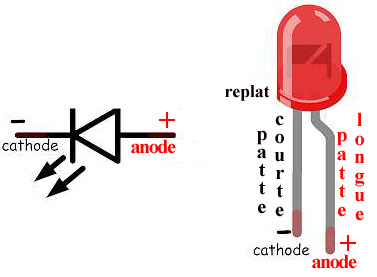
\includegraphics{images/led_schema.jpg}

\includegraphics{images/Licence.jpg}

Nous utilisons pour cette expérimentation une Raspberry Pi qui est un
nano-ordinateur disposant de broches que l'on peut relier à des
composants électroniques comme les LEDs. Nous allons utiliser le langage
\emph{python} et pour rendre les choses aussi accessibles que possible
nous n'utiliserons que des instructions simples en petit nombre. Pour
parvenir à cela ces instructions simples font appel à des programmes
invisibles pour l'utilisateur qui contrôlent les détails de
l'interaction entre la Raspberry Pi, les broches et les composants.
C'est le mode de fonctionnement standard pour développer un code, on
utilise des programmes préexistants (par exemple en programmaton
graphique comme dans Scratch ou Snap! on utilise sans s'en apercevoir
une grande quantité de programmes qui affichent les objets à l'écran,
les déplacent et les enchaînent). Tous ces programmes sont en général
regroupés dans des objets appelés bibliothèques, stockés sur le disque
de la machine et prêts à l'emploi, chaque fois qu'on en a besoin on
\emph{appelle} le programme caché qui va exécuter ce qu'on attend de lui
. Pour accéder à une librairie on utilise l'instruction :

\textbf{import} \emph{nom\_de\_la\_bibliothèque} \textbf{as}
\emph{nom\_de\_la\_bibliothèque\_utilisé\_dans\_le\_programme}

Pour appeler le programme en python on écrit :

\emph{nom\_de\_la\_bibliothèque\_utilisé\_dans\_le\_programme}\textbf{.}\emph{nom\_du\_programme\_appelé}

Les instructions \emph{import} doivent \textbf{systématiquement} figurer
en tête de chaque programme. Lors de la phase d'apprentissage elles ne
doivent être utilisées qu'\textbf{une seule fois} par programme, c'est
pour cela qu'elles sont placées dans un bloc particulier au début du
programme.

En cas de \emph{redéclaration} si la broche est dans un état \emph{"hors
service"}. La situation est réversible en utilisant la instruction
\texttt{led.dir(mraa.DIR\_IN)}, toutefois si l'indisponibilité persiste
ouvrir un \emph{terminal} depuis la page de garde du "Cahier de
programmes" et taper l'instruction \texttt{mraa-gpio\ set\ 11\ 0}.

    \subsection{Contrôler l'allumage et l'extinction d'une LED par un
programme}\label{contruxf4ler-lallumage-et-lextinction-dune-led-par-un-programme}

\subsubsection{Montage}\label{montage}

Nous allons utiliser le montage encadré ci-dessous et connecter deux
broches de la Raspberry Pi. L'identification des broche est une question
de type \emph{"troll"} car il y a plusieurs façons d'identifier ces
broches dont toutes ont des avantages et des inconvénients. Nous
utilisons dans tous les cahiers le \textbf{numéro de la broche} en
commençant en haut à gauche en descendant et en augmentant de droite à
gauche (les connecteurs USB et RJ45 de la Raspberry Pi étant orientés
vers le bas).

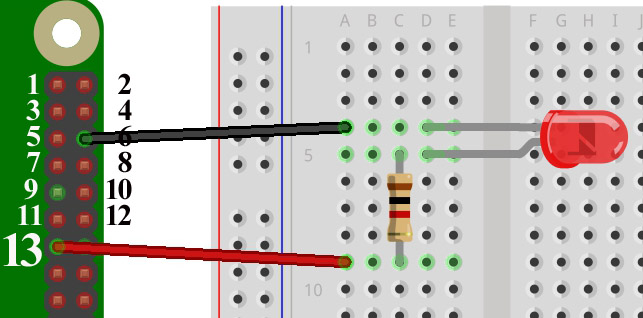
\includegraphics{images/RaspberryPi_Led_Detail.jpg}

\includegraphics{images/Licence.jpg}

Connecter la patte longue de la LED à la broche 11 en y intercalant une
résistance de 100 à 300 ohms et le fil noir à la broche 6 (GROUND).

\subsubsection{Programme}\label{programme}

Pour allumer la LED notre programme va être construit au fur ét à
mesure, il faut commencer par : * importer les programmes de la
bibliothèque mraa * déclarer l'utilisation de la broche 11

    \begin{Verbatim}[commandchars=\\\{\}]
{\color{incolor}In [{\color{incolor}1}]:} \PY{k+kn}{import} \PY{n+nn}{mraa}
        \PY{n}{led} \PY{o}{=} \PY{n}{mraa}\PY{o}{.}\PY{n}{Gpio}\PY{p}{(}\PY{l+m+mi}{11}\PY{p}{)}
\end{Verbatim}


    Toutes les broches disposent de trois modes de fonctionnenment * soit le
mode \emph{in} pour \textbf{recevoir} des données * soit le mode
\emph{out} pour \textbf{envoyer} un signal ou un courant. * soit un mode
\emph{barrière} pour bloquer tout courant (résistance infinie)

La broche 11 est reliée à l'anode (le \textbf{+}), elle doit donc
envoyer du courant, * il faut déclarer la broche 11 en mode sortie
\emph{out} On utilise l'instruction \emph{dir} (direction) qui affecte
le mode sortie (DIR\_OUT) à la LED déclarée ci dessus. L'instruction
\emph{dir} envoie un message après avoir fonctionné qui renseigne sur
l'état de la broche * l'état de la broche est indiqué par un nombre (0
correct, 7 erreur) et recueilli dans la variable status. Pour afficher
l'état décommenter la seconde ligne de ce bloc.

    \begin{Verbatim}[commandchars=\\\{\}]
{\color{incolor}In [{\color{incolor}2}]:} \PY{n}{status} \PY{o}{=} \PY{n}{led}\PY{o}{.}\PY{n}{dir}\PY{p}{(}\PY{n}{mraa}\PY{o}{.}\PY{n}{DIR\PYZus{}OUT}\PY{p}{)}
        \PY{c+c1}{\PYZsh{}print (\PYZsq{}Return status : \PYZob{}0:1d\PYZcb{}\PYZsq{}.format(status))}
\end{Verbatim}


    Pour allumer la LED on met la sortie au niveau 1 avec l'instruction
\emph{write} * l'état de la broche est fourni (0 correct, 7 erreur) et
recueilli dans la variable status. Pour afficher l'état décommenter la
seconde ligne de ce bloc.

    \begin{Verbatim}[commandchars=\\\{\}]
{\color{incolor}In [{\color{incolor}3}]:} \PY{n}{status} \PY{o}{=} \PY{n}{led}\PY{o}{.}\PY{n}{write}\PY{p}{(}\PY{l+m+mi}{1}\PY{p}{)}
        \PY{c+c1}{\PYZsh{}print (\PYZsq{}Return status : \PYZob{}0:1d\PYZcb{}\PYZsq{}.format(status))}
\end{Verbatim}


    On éteint ou on ré-éteint la LED en mettant la sortie au niveau 0 avec
l'instruction \emph{write} * l'état de la broche est fourni (0 correct,
7 erreur) et recueilli dans la variable status. Pour afficher l'état
décommenter la seconde ligne de ce bloc.

    \begin{Verbatim}[commandchars=\\\{\}]
{\color{incolor}In [{\color{incolor}4}]:} \PY{n}{status} \PY{o}{=} \PY{n}{led}\PY{o}{.}\PY{n}{write}\PY{p}{(}\PY{l+m+mi}{0}\PY{p}{)}
        \PY{c+c1}{\PYZsh{}print (\PYZsq{}Return status : \PYZob{}0:1d\PYZcb{}\PYZsq{}.format(status))}
\end{Verbatim}


    \subsection{Contrôler le clignottement d'une
LED}\label{contruxf4ler-le-clignottement-dune-led}

Pour faire clignotter la LED il est nécessaire de contrôler la durée
d'allumage et celle de l'extinction de la LED. Pour y parvenir il est
nécessaire de disposer d'instructions prenant en compte les durées,
elles sont fournies par la bibliothèque \emph{time}. On importe time
ensuite on choisit la durée d'allumage et d'extinction \textbf{en
secondes} : Exécuter le programme ci-dessous puis commenter chaque étape
Importer la bibliothèque \emph{time} Allumer la LED pendant ? secondes
Eteindre la LED pendant ? secondes ......

    \begin{Verbatim}[commandchars=\\\{\}]
{\color{incolor}In [{\color{incolor}5}]:} \PY{k+kn}{import} \PY{n+nn}{time}
        \PY{n}{led}\PY{o}{.}\PY{n}{write}\PY{p}{(}\PY{l+m+mi}{1}\PY{p}{)}
        \PY{n}{time}\PY{o}{.}\PY{n}{sleep}\PY{p}{(}\PY{l+m+mi}{1}\PY{p}{)}
        \PY{n}{led}\PY{o}{.}\PY{n}{write}\PY{p}{(}\PY{l+m+mi}{0}\PY{p}{)}
        \PY{n}{time}\PY{o}{.}\PY{n}{sleep}\PY{p}{(}\PY{l+m+mi}{1}\PY{p}{)}
        \PY{n}{led}\PY{o}{.}\PY{n}{write}\PY{p}{(}\PY{l+m+mi}{1}\PY{p}{)}
        \PY{n}{time}\PY{o}{.}\PY{n}{sleep}\PY{p}{(}\PY{l+m+mi}{1}\PY{p}{)}
        \PY{n}{led}\PY{o}{.}\PY{n}{write}\PY{p}{(}\PY{l+m+mi}{0}\PY{p}{)}
\end{Verbatim}


\begin{Verbatim}[commandchars=\\\{\}]
{\color{outcolor}Out[{\color{outcolor}5}]:} 0
\end{Verbatim}
            
    \subsubsection{Exercice 1 : Faire clignoter une
LED}\label{exercice-1-faire-clignoter-une-led}

Brancher une LED verte sur la broche 35 (GPIO 19) et la faire clignoter
10 fois; une demi seconde allumée et une demi seconde éteinte, en un
seul programme

    \begin{Verbatim}[commandchars=\\\{\}]
{\color{incolor}In [{\color{incolor} }]:} \PY{c+c1}{\PYZsh{} Taper le code ici}
\end{Verbatim}


    \subsection{Faire clignoter la Led rouge en utilisant une instruction de
répétition : la
boucle}\label{faire-clignoter-la-led-rouge-en-utilisant-une-instruction-de-ruxe9puxe9tition-la-boucle}

Comme on l'a vu ci dessus il suffit d'imposer le temps d'allumage et
d'extinction pour un obtenir un clignotement, cependant c'est très
fastidieux de répéter plusieurs fois la même séquence d'instructions. La
programmation fournit un outil qui décrit une répétition d'instructions
et permet en quelques lignes de répéter un grand nombre d'instructions
identiques. Le programme ci-dessous utilise la \emph{variable}
\textbf{i} qui : * prend la valeur 0 pour commencer : \emph{la valeur
initiale} et * se termine à 20 \emph{la valeur finale} * en augmentant
chaque fois d'une unité : \emph{le pas}

On utilise l'instruction range("valeur initiale","valeur finale","pas")

Le clignotement se compose d'une phase d'allumage pendant 0.15 s et une
phase d'extinction de 0.25 s.

    \begin{Verbatim}[commandchars=\\\{\}]
{\color{incolor}In [{\color{incolor}6}]:} \PY{k}{for} \PY{n}{i} \PY{o+ow}{in} \PY{n+nb}{range}\PY{p}{(}\PY{l+m+mi}{0}\PY{p}{,}\PY{l+m+mi}{20}\PY{p}{,}\PY{l+m+mi}{1}\PY{p}{)} \PY{p}{:}
            \PY{n}{led}\PY{o}{.}\PY{n}{write}\PY{p}{(}\PY{l+m+mi}{1}\PY{p}{)}
            \PY{n}{time}\PY{o}{.}\PY{n}{sleep}\PY{p}{(}\PY{l+m+mf}{0.15}\PY{p}{)}
            \PY{n}{led}\PY{o}{.}\PY{n}{write}\PY{p}{(}\PY{l+m+mi}{0}\PY{p}{)}
            \PY{n}{time}\PY{o}{.}\PY{n}{sleep}\PY{p}{(}\PY{l+m+mf}{0.25}\PY{p}{)}
\end{Verbatim}


    \subsubsection{Exercice 2 Instruction conditionnelle
if-else}\label{exercice-2-instruction-conditionnelle-if-else}

Modifier \emph{la valeur initiale}, \emph{la valeur finale} et \emph{le
pas} pour modifier le clignotement. (Allumage 0.35 s extinction 0.2 s 40
clignottements).

    \begin{Verbatim}[commandchars=\\\{\}]
{\color{incolor}In [{\color{incolor} }]:} \PY{k}{for} \PY{n}{i} \PY{o+ow}{in} \PY{n+nb}{range}\PY{p}{(}\PY{o}{\PYZhy{}}\PY{p}{,}\PY{o}{\PYZhy{}}\PY{p}{,}\PY{o}{\PYZhy{}}\PY{p}{)} \PY{p}{:}
            \PY{n}{led}\PY{o}{.}\PY{n}{write}\PY{p}{(}\PY{l+m+mi}{1}\PY{p}{)}
            \PY{n}{time}\PY{o}{.}\PY{n}{sleep}\PY{p}{(}\PY{o}{\PYZhy{}}\PY{o}{.}\PY{o}{\PYZhy{}}\PY{p}{)}
            \PY{n}{led}\PY{o}{.}\PY{n}{write}\PY{p}{(}\PY{l+m+mi}{0}\PY{p}{)}
            \PY{n}{time}\PY{o}{.}\PY{n}{sleep}\PY{p}{(}\PY{o}{\PYZhy{}}\PY{o}{.}\PY{o}{\PYZhy{}}\PY{p}{)}
\end{Verbatim}


    On peut modifier l'instruction qui est répétée en ajoutant des tests qui
permettent de fixer le moment ou le type de clignotement change. Ici on
change tous les 10 clignotements.

    \begin{Verbatim}[commandchars=\\\{\}]
{\color{incolor}In [{\color{incolor}7}]:} \PY{k}{for} \PY{n}{i} \PY{o+ow}{in} \PY{n+nb}{range}\PY{p}{(}\PY{l+m+mi}{0}\PY{p}{,}\PY{l+m+mi}{30}\PY{p}{,}\PY{l+m+mi}{1}\PY{p}{)} \PY{p}{:}
            \PY{k}{if} \PY{p}{(}\PY{n}{i} \PY{o}{\PYZlt{}} \PY{l+m+mi}{10}\PY{p}{)} \PY{p}{:}
                \PY{n}{led}\PY{o}{.}\PY{n}{write}\PY{p}{(}\PY{l+m+mi}{1}\PY{p}{)}
                \PY{n}{time}\PY{o}{.}\PY{n}{sleep}\PY{p}{(}\PY{l+m+mi}{1}\PY{p}{)}
                \PY{n}{led}\PY{o}{.}\PY{n}{write}\PY{p}{(}\PY{l+m+mi}{0}\PY{p}{)}
                \PY{n}{time}\PY{o}{.}\PY{n}{sleep}\PY{p}{(}\PY{l+m+mi}{1}\PY{p}{)}
            \PY{k}{elif} \PY{p}{(}\PY{n}{i} \PY{o}{\PYZgt{}}\PY{o}{=} \PY{l+m+mi}{10} \PY{o+ow}{and} \PY{n}{i} \PY{o}{\PYZlt{}} \PY{l+m+mi}{20}\PY{p}{)} \PY{p}{:}
                \PY{n}{led}\PY{o}{.}\PY{n}{write}\PY{p}{(}\PY{l+m+mi}{1}\PY{p}{)}
                \PY{n}{time}\PY{o}{.}\PY{n}{sleep}\PY{p}{(}\PY{l+m+mf}{0.2}\PY{p}{)}
                \PY{n}{led}\PY{o}{.}\PY{n}{write}\PY{p}{(}\PY{l+m+mi}{0}\PY{p}{)}
                \PY{n}{time}\PY{o}{.}\PY{n}{sleep}\PY{p}{(}\PY{l+m+mf}{0.2}\PY{p}{)}
            \PY{k}{else} \PY{p}{:}
                \PY{n}{led}\PY{o}{.}\PY{n}{write}\PY{p}{(}\PY{l+m+mi}{1}\PY{p}{)}
                \PY{n}{time}\PY{o}{.}\PY{n}{sleep}\PY{p}{(}\PY{l+m+mf}{0.05}\PY{p}{)}
                \PY{n}{led}\PY{o}{.}\PY{n}{write}\PY{p}{(}\PY{l+m+mi}{0}\PY{p}{)}
                \PY{n}{time}\PY{o}{.}\PY{n}{sleep}\PY{p}{(}\PY{l+m+mf}{0.05}\PY{p}{)}
\end{Verbatim}


    \subsubsection{Exercice 3}\label{exercice-3}

Décrivez un mode de clignotement composé de plusieurs phases sur le
modèle ci-dessus et écrivez le programme correspondant dans le bloc
ci-dessous.

    \begin{Verbatim}[commandchars=\\\{\}]
{\color{incolor}In [{\color{incolor} }]:} \PY{k}{for} \PY{n}{i} \PY{o+ow}{in} \PY{n+nb}{range}\PY{p}{(}\PY{o}{\PYZhy{}}\PY{p}{,}\PY{o}{\PYZhy{}}\PY{p}{,}\PY{o}{\PYZhy{}}\PY{p}{)} \PY{p}{:}
            \PY{k}{if} \PY{p}{(}\PY{o}{\PYZhy{}} \PY{o}{\PYZlt{}} \PY{o}{\PYZhy{}}\PY{p}{)} \PY{p}{:}
                \PY{n}{led}\PY{o}{.}\PY{n}{write}\PY{p}{(}\PY{l+m+mi}{1}\PY{p}{)}
                \PY{n}{time}\PY{o}{.}\PY{n}{sleep}\PY{p}{(}\PY{o}{\PYZhy{}}\PY{o}{.}\PY{o}{\PYZhy{}}\PY{p}{)}
                \PY{n}{led}\PY{o}{.}\PY{n}{write}\PY{p}{(}\PY{l+m+mi}{0}\PY{p}{)}
                \PY{n}{time}\PY{o}{.}\PY{n}{sleep}\PY{p}{(}\PY{o}{\PYZhy{}}\PY{o}{.}\PY{o}{\PYZhy{}}\PY{p}{)}
            \PY{k}{elif} \PY{p}{(}\PY{p}{)}\PY{p}{:}
            
            \PY{k}{else} \PY{p}{:}
            
\end{Verbatim}



    % Add a bibliography block to the postdoc
    
    
    
    \end{document}
